% =====================================================================
%  MCMP117 -- Fundamentals of Operating Systems
%  Week 5 Course Notes: CPU Scheduling Algorithms & Process Synchronisation
%  Compile with XeLaTeX (twice):  xelatex MCMP117_Week5_Notes.tex
%  Needs ./figures/ and the ../code/ folder.
% =====================================================================
\documentclass[11pt,a4paper]{article}
\newcommand{\weeknum}{5}
% ---------- Page & fonts ---------------------------------------------
\usepackage[a4paper,margin=2.3cm,headheight=15pt]{geometry}
\usepackage{fontspec}
\IfFontExistsTF{Calibri}{\setmainfont{Calibri}}{\setmainfont{Carlito}}
\IfFontExistsTF{Cambria}{\newfontfamily\headfont{Cambria}}{\newfontfamily\headfont{Caladea}}
\IfFontExistsTF{Consolas}{\setmonofont[Scale=0.95]{Consolas}}{\setmonofont[Scale=0.88]{DejaVu Sans Mono}}
\usepackage{amsmath,amssymb}
\usepackage{microtype}
\linespread{1.12}
\setlength{\parskip}{0.55em}
\setlength{\parindent}{0pt}

% ---------- Colours (course design system) ----------------------------
\usepackage{xcolor}
\definecolor{dark}{HTML}{212121}
\definecolor{charcoal}{HTML}{36454F}
\definecolor{slate}{HTML}{50808E}
\definecolor{mint}{HTML}{02C39A}
\definecolor{mintdeep}{HTML}{028090}
\definecolor{light}{HTML}{F2F2F2}
\definecolor{muted}{HTML}{6B7679}

% ---------- Packages ---------------------------------------------------
\usepackage{graphicx}
\usepackage{float}
\usepackage{needspace}
\graphicspath{{figures/}}
\usepackage[font=small,labelfont={bf,color=mintdeep},justification=centering]{caption}
\usepackage{booktabs,longtable,array,tabularx}
\usepackage{enumitem}
\setlist{itemsep=0.25em,topsep=0.3em}
\usepackage{tikz}
\usetikzlibrary{arrows.meta,positioning,calc,shapes.geometric}
\usepackage{pgfplots}
\pgfplotsset{compat=1.17}
\usepackage[most]{tcolorbox}
\usepackage{titlesec}
\usepackage{fancyhdr}
\usepackage{xurl}
\usepackage[colorlinks=true,linkcolor=mintdeep,urlcolor=mintdeep,citecolor=mintdeep]{hyperref}

% ---------- Headings ----------------------------------------------------
\titleformat{\section}{\headfont\Large\bfseries\color{charcoal}}{\color{mint}\thesection}{0.7em}{}
\titleformat{\subsection}{\headfont\large\bfseries\color{charcoal}}{\color{mintdeep}\thesubsection}{0.6em}{}
\titleformat{\subsubsection}{\headfont\normalsize\bfseries\color{mintdeep}}{}{0em}{}
\titlespacing*{\section}{0pt}{1.6em}{0.6em}
\titlespacing*{\subsection}{0pt}{1.2em}{0.4em}

% ---------- Header / footer -----------------------------------------------
\pagestyle{fancy}
\fancyhf{}
\fancyhead[L]{\small\color{muted}MCMP117 --- Fundamentals of Operating Systems}
\fancyhead[R]{\small\color{muted}Week \weeknum{} Notes}
\fancyfoot[C]{\small\color{muted}\thepage}
\renewcommand{\headrulewidth}{0pt}

% ---------- Boxes ---------------------------------------------------------
\newtcolorbox{keyidea}[1][Key idea]{enhanced,breakable,colback=charcoal,colframe=charcoal,
  coltext=white,fonttitle=\headfont\bfseries\color{mint},title={#1},
  attach title to upper={\par\smallskip},boxrule=0pt,arc=3pt,left=10pt,right=10pt,top=8pt,bottom=8pt}
\newtcolorbox{example}[1][Worked example]{enhanced,colback=light,colframe=light,
  fonttitle=\headfont\bfseries\color{mintdeep},title={#1},attach title to upper={\par\smallskip},
  boxrule=0pt,arc=3pt,left=10pt,right=10pt,top=8pt,bottom=8pt}
\newtcolorbox{tryit}[1][Try it yourself]{enhanced,breakable,colback=white,colframe=mint,
  fonttitle=\headfont\bfseries\color{mintdeep},title={#1},attach title to upper={\par\smallskip},
  boxrule=0.8pt,arc=3pt,left=10pt,right=10pt,top=8pt,bottom=8pt}
\newtcolorbox{histnote}[1][Historical note]{enhanced,breakable,colback=white,colframe=slate!40,
  fonttitle=\headfont\bfseries\color{slate},title={#1},attach title to upper={\par\smallskip},
  boxrule=0.5pt,arc=3pt,left=10pt,right=10pt,top=8pt,bottom=8pt,fontupper=\small}

% Photo helper: fits image inside a box, never distorted (keepaspectratio)
\newcommand{\photo}[3]{\includegraphics[width=#1,height=#2,keepaspectratio]{#3}}

\newcommand{\term}[1]{\textbf{\color{mintdeep}#1}}
\newcommand{\cmd}[1]{\texttt{#1}}


% ---------- Code listings ----------------------------------------------------
\usepackage{listings}
\lstdefinestyle{course}{
  basicstyle=\ttfamily\small, columns=fullflexible, keepspaces=true,
  backgroundcolor=\color{dark}, rulecolor=\color{dark}, frame=single, framesep=6pt,
  xleftmargin=8pt, xrightmargin=8pt, aboveskip=0.8em, belowskip=0.6em,
  basicstyle=\ttfamily\small\color{light},
  keywordstyle=\color{mint}\bfseries, commentstyle=\color{white!60}\itshape,
  stringstyle=\color{orange!70!yellow}, numberstyle=\tiny\color{muted},
  numbers=left, numbersep=10pt, showstringspaces=false, breaklines=true,
  tabsize=4, upquote=true}
\lstdefinestyle{term}{style=course, numbers=none, keywordstyle=\color{light},
  commentstyle=\color{white!60}, stringstyle=\color{light}}
\lstset{style=course,language=C}
\usepackage{textcomp}

\begin{document}
% ============================ Week 5 body ============================
\lstset{basicstyle=\ttfamily\footnotesize\color{light}}
% Gantt-chart helpers (colours match the slides)
\definecolor{amber}{HTML}{C98A1B}
\colorlet{colP1}{mint}\colorlet{txtP1}{dark}
\colorlet{colP2}{slate}\colorlet{txtP2}{white}
\colorlet{colP3}{amber}\colorlet{txtP3}{white}
\colorlet{colP4}{charcoal}\colorlet{txtP4}{white}
\colorlet{colA}{mint}\colorlet{txtA}{dark}
\colorlet{colB}{slate}\colorlet{txtB}{white}
\colorlet{colC}{amber}\colorlet{txtC}{white}
\colorlet{colD}{charcoal}\colorlet{txtD}{white}
\colorlet{colL}{charcoal}\colorlet{txtL}{white}
\colorlet{colS}{amber}\colorlet{txtS}{white}
% \gantt{unit in cm per ms}{P/start/end, ...}
\newcommand{\gantt}[2]{%
\begin{tikzpicture}[x=#1cm,y=1cm]
\foreach \p/\a/\b in {#2} {
  \fill[col\p] (\a,0) rectangle (\b,0.62);
  \draw[white,line width=1.2pt] (\a,0) -- (\a,0.62);
  \node[font=\small\bfseries,text=txt\p] at ({(\a+\b)/2},0.31) {\p};
  \draw[muted] (\a,0) -- (\a,-0.1) node[below,font=\scriptsize,text=muted,inner sep=1.5pt] {\a};
  \draw[muted] (\b,0) -- (\b,-0.1) node[below,font=\scriptsize,text=muted,inner sep=1.5pt] {\b};
}
\end{tikzpicture}}

\thispagestyle{empty}
\begin{tcolorbox}[enhanced,colback=dark,colframe=dark,arc=0pt,boxrule=0pt,
  left=18pt,right=18pt,top=20pt,bottom=20pt,coltext=white]
{\small\color{mint}\textsc{MCMP117 \,·\, Week 5 \,·\, Course Notes}}\par\medskip
{\headfont\fontsize{26}{30}\selectfont\bfseries Fundamentals of Operating Systems}\par\medskip
{\large CPU Scheduling Algorithms \& Process Synchronisation}\par\smallskip
{\small\itshape\color{white!70} Who runs next, and how do threads share data without breaking it?}
\end{tcolorbox}

\vspace{0.4em}
{\small
\textbf{Instructor:} Asst.\ Prof.\ Dr.\ (Ph.D.) Hasan Oğuz\\
Head of the Electronical Communication Technology Programme, Vocational School\\
Istanbul Okan University\par}

\vspace{0.8em}
\begin{keyidea}[What you should be able to do after this week]
\begin{enumerate}[leftmargin=1.4em]
  \item Draw the Gantt chart of a job set under FCFS, SJF, SRTF, priority and Round Robin scheduling, and compute the waiting, turnaround and response time of every process.
  \item Explain the convoy effect, why SJF minimises the average waiting time, and how the next CPU burst is predicted by exponential averaging.
  \item Explain starvation and aging, and the trade-off in choosing the Round Robin time quantum.
  \item Describe, at overview level, multilevel feedback queues and the fair scheduler used by Linux.
  \item Explain a race condition using the load--add--store sequence of \cmd{counter++}; state the critical-section problem and its three requirements, and describe Peterson's solution, atomic instructions, mutex locks and semaphores.
  \item Solve the bounded-buffer problem with semaphores and recognise a simple deadlock.
  \item Read, compile and run small \texttt{pthreads} programs that show a race and its fix.
\end{enumerate}
\end{keyidea}

\setcounter{tocdepth}{1}
\tableofcontents

% =====================================================================
\section{Recap and the Running Example}

Last week we met the \term{CPU scheduler}, which chooses one process from the ready queue, and the \term{dispatcher}, which actually gives it the CPU (context switch, switch to user mode, jump to the right instruction). Scheduling can be \term{non-preemptive} (a process keeps the CPU until it terminates or blocks for I/O) or \term{preemptive} (the OS may take the CPU away, typically on a timer interrupt or when a more important process becomes ready). We judge a schedule by the following criteria, where every time is measured for one process:
\begin{align*}
T_{\text{turnaround}} &= T_{\text{completion}} - T_{\text{arrival}},\\
T_{\text{waiting}} &= T_{\text{turnaround}} - T_{\text{burst}},\\
T_{\text{response}} &= T_{\text{first run}} - T_{\text{arrival}}.
\end{align*}
The waiting time is the total time a process spends \emph{in the ready queue}. For a non-preemptive algorithm a process runs in one piece, so its waiting time equals its response time. CPU utilisation and throughput should be as high as possible; turnaround, waiting and response time as low as possible.

\subsection{One job set for every algorithm}
\label{sec:jobs}

To compare algorithms fairly we use the \emph{same} four processes throughout Part~1. All times are in milliseconds (ms).

\begin{center}
\renewcommand{\arraystretch}{1.25}
\begin{tabular}{@{}cccc@{}}
\toprule
\textbf{Process} & \textbf{Arrival time} & \textbf{CPU burst} & \textbf{Priority} \\
\midrule
P1 & 0 & 7 & 3 \\
P2 & 2 & 4 & 1 \\
P3 & 4 & 1 & 4 \\
P4 & 5 & 4 & 2 \\
\bottomrule
\end{tabular}
\end{center}

Conventions (state them in every exam answer, because textbooks differ):
\begin{itemize}
  \item Context-switch time is taken as $0$; we count the number of switches separately.
  \item Ties are broken by arrival time, then by process name.
  \item A \emph{smaller} priority number means a \emph{higher} priority.
  \item In Round Robin, a process that arrives at the same instant as a quantum expires enters the ready queue \emph{before} the preempted process.
\end{itemize}

The total CPU work is $7+4+1+4=16$ ms and the CPU is never idle, so every schedule below ends at $t=16$. A \term{Gantt chart} is a time line divided into boxes; each box shows which process uses the CPU during that interval.

Every number in these notes and on the slides was computed by a short Python program in the \texttt{code/} folder, \texttt{sched\_check.py}. Run \cmd{python3 sched\_check.py} to print all Gantt charts and tables, or edit its list \texttt{JOBS} to try your own job set.

% =====================================================================
\section{First-Come, First-Served (FCFS)}

The simplest policy: the ready queue is a FIFO (first-in, first-out) queue, and the process that arrived first gets the CPU and keeps it until it finishes or blocks. FCFS is non-preemptive.

\begin{center}
\gantt{0.95}{P1/0/7, P2/7/11, P3/11/12, P4/12/16}
\end{center}

\begin{center}
\renewcommand{\arraystretch}{1.2}
\begin{tabular}{@{}lcccccc@{}}
\toprule
\textbf{Process} & \textbf{Arrival} & \textbf{Burst} & \textbf{Finish} & \textbf{Turnaround} & \textbf{Waiting} & \textbf{Response}\\
\midrule
P1 & 0 & 7 & 7 & 7 & 0 & 0\\
P2 & 2 & 4 & 11 & 9 & 5 & 5\\
P3 & 4 & 1 & 12 & 8 & 7 & 7\\
P4 & 5 & 4 & 16 & 11 & 7 & 7\\
\midrule
\textbf{Average} & & & & $8.75$ & $4.75$ & $4.75$\\
\bottomrule
\end{tabular}
\end{center}

For example, P3 arrives at $t=4$, starts at $t=11$ and finishes at $t=12$: $T_{\text{turnaround}} = 12-4 = 8$ ms and $T_{\text{waiting}} = 8-1 = 7$ ms. The average waiting time is $(0+5+7+7)/4 = 4.75$ ms.

\subsection{The convoy effect}

FCFS is fair in the ``queue at the bank'' sense, but the average waiting time depends heavily on the order in which processes happen to arrive. Take three jobs that all arrive at $t=0$ with bursts of $24$, $3$ and $3$ ms.

\begin{center}
\begin{tabular}{@{}r@{\quad}l@{}}
\small Order A: & \gantt{0.42}{P1/0/24, P2/24/27, P3/27/30}\\[0.6em]
\small Order B: & \gantt{0.42}{P2/0/3, P3/3/6, P1/6/30}
\end{tabular}
\end{center}

\begin{align*}
\text{Order A:}\quad \overline{T}_{\text{waiting}} &= \frac{0 + 24 + 27}{3} = \frac{51}{3} = 17\ \text{ms},\\
\text{Order B:}\quad \overline{T}_{\text{waiting}} &= \frac{0 + 3 + 6}{3} = \frac{9}{3} = 3\ \text{ms}.
\end{align*}

Same jobs, same algorithm, almost six times less waiting. When many short, I/O-bound processes are stuck behind one long CPU-bound process, the whole system slows down, like cars behind a slow truck on a mountain road. This is the \term{convoy effect}: the I/O devices sit idle while the short jobs wait, and then the CPU sits idle while they all do I/O.

% =====================================================================
\section{Shortest-Job-First Scheduling}

Order B above suggests a better rule: \emph{run the shortest job first}. Strictly, the rule looks at the length of the \emph{next CPU burst}, not of the whole job, so a more accurate name would be ``shortest-next-CPU-burst''.

\subsection{Non-preemptive SJF}

Whenever the CPU becomes free, choose the ready process with the shortest next burst; once started, it runs to completion.

\begin{center}
\gantt{0.95}{P1/0/7, P3/7/8, P2/8/12, P4/12/16}
\end{center}

At $t=0$ only P1 is ready, so it runs to $t=7$. At $t=7$ the ready queue holds P2 (4 ms), P3 (1 ms) and P4 (4 ms); P3 is shortest. At $t=8$, P2 and P4 tie at $4$ ms and P2 arrived first.

The waiting times are P1 $0$, P2 $12-2-4=6$, P3 $8-4-1=3$ and P4 $16-5-4=7$ ms; the turnaround times are $7$, $10$, $4$ and $11$ ms.


The average waiting time falls from $4.75$ ms (FCFS) to $4$ ms. Note the remaining weakness: P1 started at $t=0$ simply because nobody else was there, and then the very short P3 had to wait for it.

\subsection{Preemptive SJF: shortest-remaining-time-first (SRTF)}

In the preemptive version, every time a new process arrives the scheduler compares its burst with the \emph{remaining} time of the running process; if the newcomer is shorter, it takes the CPU.

\begin{center}
\gantt{0.95}{P1/0/2, P2/2/4, P3/4/5, P2/5/7, P4/7/11, P1/11/16}
\end{center}

\begin{itemize}
  \item $t=2$: P2 arrives needing $4$ ms; P1 still needs $7-2=5$ ms. Since $4<5$, P1 is preempted.
  \item $t=4$: P3 arrives needing $1$ ms; P2 still needs $2$ ms. P2 is preempted.
  \item $t=5$: P3 is done. Remaining times: P2 $2$, P4 $4$, P1 $5$. So P2 runs $5$--$7$, then P4 $7$--$11$, then P1 $11$--$16$.
\end{itemize}

\begin{center}
\renewcommand{\arraystretch}{1.2}
\begin{tabular}{@{}lcccccc@{}}
\toprule
\textbf{Process} & \textbf{Arrival} & \textbf{Burst} & \textbf{Finish} & \textbf{Turnaround} & \textbf{Waiting} & \textbf{Response}\\
\midrule
P1 & 0 & 7 & 16 & 16 & 9 & 0\\
P2 & 2 & 4 & 7 & 5 & 1 & 0\\
P3 & 4 & 1 & 5 & 1 & 0 & 0\\
P4 & 5 & 4 & 11 & 6 & 2 & 2\\
\midrule
\textbf{Average} & & & & $7$ & $3$ & $0.5$\\
\bottomrule
\end{tabular}
\end{center}

With preemption a process may run in several pieces, so we compute the waiting time from the formula rather than by adding up gaps: P1 finishes at $16$, so $T_{\text{waiting}}(\text{P1}) = (16-0) - 7 = 9$ ms (check: P1 waited from $2$ to $11$, i.e.\ $9$ ms). The average waiting time is $(9+1+0+2)/4 = 3$ ms, the best value of the day; the long job P1 pays for the speed of the short ones.

\subsection{Why shortest-first is optimal}

\begin{keyidea}[Optimality of SJF]
If all jobs are available at the same time, running them in order of increasing burst length gives the minimum possible average waiting time. When jobs arrive at different times, SRTF gives the minimum (if context switches are free).
\end{keyidea}

The proof is an \emph{exchange argument}. Consider any schedule in which a longer job $L$ runs immediately before a shorter job $S$ ($L > S$), starting at some time $t_0$. Swap the two:
\begin{itemize}
  \item Every job before the pair starts at the same time as before; every job after the pair also starts at the same time, because $L+S$ is unchanged.
  \item Inside the pair, the waiting times were $t_0$ (for $L$) and $t_0+L$ (for $S$); after the swap they are $t_0$ and $t_0+S$.
\end{itemize}
The total waiting time therefore decreases by $L-S>0$. Any schedule with a longer job before a shorter one can be improved, so the shortest-first order is optimal. In the convoy example, order B is exactly the shortest-first order.

\subsection{The catch: predicting the next CPU burst}

SJF needs the length of the next CPU burst \emph{before} the process runs. For long-term batch scheduling, users could be asked to estimate the run time of their job; for CPU scheduling there is no way to know. The OS can only \emph{predict}, assuming that the next burst will be similar to recent ones. The standard predictor is the \term{exponential average}
\[
\tau_{n+1} = \alpha\, t_n + (1-\alpha)\, \tau_n, \qquad 0 \le \alpha \le 1,
\]
where $t_n$ is the measured length of the $n$-th burst and $\tau_n$ is the value that had been predicted for it. Expanding the recursion shows where the name comes from:
\[
\tau_{n+1} = \alpha t_n + (1-\alpha)\alpha t_{n-1} + (1-\alpha)^2 \alpha t_{n-2} + \dots + (1-\alpha)^{n+1}\tau_0 .
\]
Since $1-\alpha<1$, older bursts get exponentially smaller weights. With $\alpha=0$ the prediction never changes (recent history is ignored); with $\alpha=1$ only the last burst counts. A common choice is $\alpha = 1/2$.

\begin{example}[Exponential averaging, $\alpha = 1/2$, $\tau_0 = 10$ ms]
The process has actual bursts $t_0, t_1, \dots = 6, 4, 6, 4, 13, 13, 13$ ms. The first two steps:
\begin{align*}
\tau_1 &= \tfrac12 \cdot 6 + \tfrac12 \cdot 10 = 8\ \text{ms},\\
\tau_2 &= \tfrac12 \cdot 4 + \tfrac12 \cdot 8 = 6\ \text{ms}.
\end{align*}
Continuing in the same way:
\begin{center}
\renewcommand{\arraystretch}{1.2}
\begin{tabular}{@{}lcccccccc@{}}
\toprule
$n$ & 0 & 1 & 2 & 3 & 4 & 5 & 6 & 7\\
\midrule
actual burst $t_n$ (ms) & 6 & 4 & 6 & 4 & 13 & 13 & 13 & ?\\
prediction $\tau_n$ (ms) & 10 & 8 & 6 & 6 & 5 & 9 & 11 & 12\\
\bottomrule
\end{tabular}
\end{center}
When the behaviour of the process changes (bursts jump to $13$ ms), the prediction follows with a delay: $5 \to 9 \to 11 \to 12$. This lag is the price of smoothing out random fluctuations.
\end{example}


% =====================================================================
\section{Priority Scheduling}

Each process is given a \term{priority}, and the CPU goes to the ready process with the highest priority. In this course (as in Linux and in Silberschatz) a smaller number means a higher priority. SJF is the special case in which the priority is the predicted burst length. Priority scheduling can be non-preemptive or preemptive.

\begin{center}
\begin{tabular}{@{}r@{\quad}l@{}}
\small Non-preemptive: & \gantt{0.8}{P1/0/7, P2/7/11, P4/11/15, P3/15/16}\\[0.6em]
\small Preemptive: & \gantt{0.8}{P1/0/2, P2/2/6, P4/6/10, P1/10/15, P3/15/16}
\end{tabular}
\end{center}

In the preemptive version P2 (priority $1$) takes the CPU from P1 (priority $3$) as soon as it arrives at $t=2$ and runs to $6$; then P4 (priority $2$, arrived at $5$) runs $6$--$10$; P1 finishes $10$--$15$; P3 runs last.

\begin{center}
\renewcommand{\arraystretch}{1.2}
\begin{tabular}{@{}lccccc@{}}
\toprule
& & \multicolumn{2}{c}{\textbf{Non-preemptive}} & \multicolumn{2}{c}{\textbf{Preemptive}}\\
\cmidrule(lr){3-4}\cmidrule(lr){5-6}
\textbf{Process} & \textbf{Priority} & \textbf{Waiting} & \textbf{Response} & \textbf{Waiting} & \textbf{Response}\\
\midrule
P1 & 3 & 0 & 0 & 8 & 0\\
P2 & 1 & 5 & 5 & 0 & 0\\
P3 & 4 & 11 & 11 & 11 & 11\\
P4 & 2 & 6 & 6 & 1 & 1\\
\midrule
\textbf{Average} & & $5.5$ & $5.5$ & $5$ & $3$\\
\bottomrule
\end{tabular}
\end{center}

The average turnaround times are $9.5$ ms (non-preemptive) and $9$ ms (preemptive). Priority scheduling does not try to minimise averages: it serves \emph{importance}. Priorities can be \emph{internal} (computed by the OS from measurable quantities such as memory needs or the ratio of I/O to CPU bursts) or \emph{external} (set from outside: the importance of the job, the department that pays for it).

\subsection{Starvation and aging}

P3, with the lowest priority, waited $11$ ms in both versions. In a busy system where higher-priority processes keep arriving, a low-priority process may \emph{never} run. This is called \term{starvation} or \emph{indefinite blocking}.

\begin{histnote}[A job that waited six years]
According to a widely repeated story, when the IBM 7094 at MIT was shut down in 1973, the operators found a low-priority process that had been submitted in 1967 and had never been run. Whether or not every detail is true, it illustrates the problem well.
\end{histnote}

The standard cure is \term{aging}: gradually increase the priority of a process the longer it waits. For example, if priorities range from $127$ (lowest) to $0$ (highest) and a waiting process gains one priority level every second, even a process that starts at $127$ reaches priority $0$ after at most
\[
127 \times 1\ \text{s} = 127\ \text{s} = 2\ \text{min}\ 7\ \text{s}.
\]
Aging turns ``maybe never'' into ``within a bounded time''. We will meet the same idea again as the \emph{bounded-waiting} requirement in Section~\ref{sec:cs}.

% =====================================================================
\section{Round Robin Scheduling}

\term{Round Robin} (RR) is FCFS with preemption, designed for time-sharing systems. A small unit of time, the \term{time quantum} (or time slice) $q$, is defined, typically $10$--$100$ ms. The ready queue is treated as a circular FIFO queue:
\begin{enumerate}[leftmargin=1.4em]
  \item The scheduler takes the process at the head of the queue and sets a timer to interrupt after $q$.
  \item If the CPU burst ends before $q$ (the process finishes or blocks for I/O), the process leaves the CPU voluntarily and the next one starts at once.
  \item If the timer goes off first, the process is preempted and put at the \emph{tail} of the ready queue.
\end{enumerate}

\begin{figure}[H]
\centering
\begin{tikzpicture}[q/.style={rectangle,rounded corners=2pt,minimum width=1.0cm,minimum height=0.75cm,font=\small\bfseries},
  arr/.style={-{Stealth[length=2.5mm]},thick,slate}]
\node[q,fill=charcoal,text=white] (a) at (0,0) {P4};
\node[q,fill=amber,text=white] (b) at (1.2,0) {P3};
\node[q,fill=slate,text=white] (c) at (2.4,0) {P2};
\node[font=\footnotesize\itshape,text=muted] at (1.2,0.7) {ready queue (tail \dots\ head)};
\node[rectangle,rounded corners=3pt,fill=mint,minimum width=2.2cm,minimum height=1.1cm,align=center,font=\small] (cpu) at (5.2,0) {\textbf{CPU}\\running P1};
\draw[arr] (c) -- (cpu);
\draw[arr] (cpu.east) -- ++(1.3,0) node[right,font=\footnotesize,text=slate,align=left] {finished or\\blocked for I/O};
\draw[-{Stealth[length=2.5mm]},thick,red!60!black] (cpu.south) -- ++(0,-0.7) -| (a.south) node[pos=0.25,below,font=\footnotesize] {quantum expired (timer interrupt): back to the tail};
\end{tikzpicture}
\caption{Round Robin.}
\end{figure}

With $n$ processes in the ready queue, each gets $1/n$ of the CPU time in chunks of at most $q$, and no process waits more than $(n-1)\,q$ before its next turn. This bound is what makes RR good for response time.

\subsection{Worked example: $q = 4$ ms}

\begin{center}
\gantt{0.95}{P1/0/4, P2/4/8, P3/8/9, P1/9/12, P4/12/16}
\end{center}

Follow the ready queue (head on the left):
\begin{itemize}
  \item $t=0$: only P1; it runs for a full quantum, $0$--$4$.
  \item $t=4$: P2 (arrived at $2$) and P3 (arrived at $4$) are queued; P1 joins at the tail (our convention: P3, arriving exactly at $4$, goes before P1). Queue: P2, P3, P1.
  \item $t=8$: P2 has used its $4$ ms and is finished. P4 arrived at $5$. Queue: P3, P1, P4.
  \item $t=9$: P3 finished after $1$ ms. P1 needs $3$ more ms and finishes at $12$; then P4 runs $12$--$16$.
\end{itemize}

\begin{center}
\renewcommand{\arraystretch}{1.2}
\begin{tabular}{@{}lcccccc@{}}
\toprule
\textbf{Process} & \textbf{Arrival} & \textbf{Burst} & \textbf{Finish} & \textbf{Turnaround} & \textbf{Waiting} & \textbf{Response}\\
\midrule
P1 & 0 & 7 & 12 & 12 & 5 & 0\\
P2 & 2 & 4 & 8 & 6 & 2 & 2\\
P3 & 4 & 1 & 9 & 5 & 4 & 4\\
P4 & 5 & 4 & 16 & 11 & 7 & 7\\
\midrule
\textbf{Average} & & & & $8.5$ & $4.5$ & $3.25$\\
\bottomrule
\end{tabular}
\end{center}

\subsection{Worked example: $q = 2$ ms}

\begin{center}
\gantt{0.95}{P1/0/2, P2/2/4, P1/4/6, P3/6/7, P2/7/9, P4/9/11, P1/11/13, P4/13/15, P1/15/16}
\end{center}

\begin{center}
\renewcommand{\arraystretch}{1.15}
\begin{tabular}{@{}cll@{}}
\toprule
\textbf{Time} & \textbf{Event} & \textbf{Ready queue afterwards (head first)}\\
\midrule
0 & P1 starts & --- \\
2 & P2 arrived; P1's quantum expires & P2, P1 \\
4 & P3 arrived; P2's quantum expires & P1, P3, P2 \\
6 & P4 arrived at 5; P1's quantum expires & P3, P2, P4, P1 \\
7 & P3 finishes (1 ms burst) & P2, P4, P1 \\
9 & P2 finishes & P4, P1 \\
11 & P4's quantum expires & P1, P4 \\
13 & P1's quantum expires & P4, P1 \\
15 & P4 finishes; P1 runs its last 1 ms & --- \\
\bottomrule
\end{tabular}
\end{center}

Finishing times are P1 $16$, P2 $9$, P3 $7$, P4 $15$, so the waiting times are $9$, $3$, $2$ and $6$ ms and the response times $0$, $0$, $2$ and $4$ ms (averages: waiting $5$, turnaround $9$, response $1.5$ ms).


Compared with $q=4$: the average response time improves from $3.25$ to $1.5$ ms, but the average waiting time grows from $4.5$ to $5$ ms and the number of context switches doubles from $4$ to $8$.

\subsection{Choosing the time quantum}

\begin{center}
\renewcommand{\arraystretch}{1.2}
\begin{tabular}{@{}cccc@{}}
\toprule
\textbf{Quantum $q$} & \textbf{Avg waiting (ms)} & \textbf{Avg response (ms)} & \textbf{Context switches}\\
\midrule
1 ms & $5.5$ & $0.75$ & 14\\
2 ms & $5$ & $1.5$ & 8\\
4 ms & $4.5$ & $3.25$ & 4\\
8 ms & $4.75$ & $4.75$ & 3\\
\bottomrule
\end{tabular}
\end{center}

\begin{itemize}
  \item \textbf{$q$ too large:} RR degenerates into FCFS. With $q = 8$ ms, which is longer than every burst in our job set, the schedule is \emph{identical} to FCFS.
  \item \textbf{$q$ too small:} the CPU spends a large share of its time switching. If each switch costs $s$, then each quantum of useful work $q$ costs one switch, and the fraction of CPU time lost is
\[
\frac{s}{q+s}.
\]
With a (deliberately pessimistic) switch cost of $s=0.1$ ms this gives $9.1\%$ for $q=1$ ms, $2.4\%$ for $q=4$ ms, $1.0\%$ for $q=10$ ms and $0.1\%$ for $q=100$ ms.
\end{itemize}

Real context switches cost a few microseconds, plus an indirect cost: the caches and the TLB are ``cold'' for the newly scheduled process. A common rule of thumb is to choose $q$ so that about $80\%$ of CPU bursts are shorter than $q$; interactive processes then usually finish their burst within one quantum.

% =====================================================================
\section{Multilevel Queues and Real Schedulers (Overview)}

\subsection{Multilevel queue and multilevel feedback queue}

Real systems combine several algorithms. In a \term{multilevel queue} scheduler the ready queue is split into several queues, for example \emph{foreground} (interactive) processes scheduled by RR and \emph{background} (batch) processes scheduled by FCFS, with fixed priority between the queues. A process stays in its queue permanently.

A \term{multilevel feedback queue} (MLFQ) lets processes move between queues according to their behaviour. A classic example has three queues:

\begin{figure}[H]
\centering
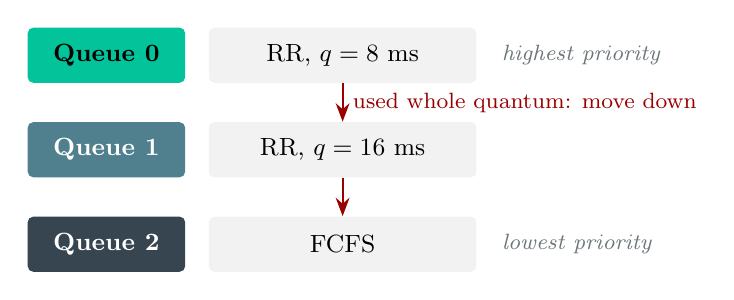
\begin{tikzpicture}[q/.style={rectangle,rounded corners=2pt,minimum width=2.0cm,minimum height=0.7cm,font=\small\bfseries},
 p/.style={rectangle,rounded corners=2pt,fill=light,minimum width=3.4cm,minimum height=0.7cm,font=\small}]
\node[q,fill=mint] (q0) at (0,0) {Queue 0}; \node[p] (p0) at (3,0) {RR, $q = 8$ ms};
\node[q,fill=slate,text=white] (q1) at (0,-1.2) {Queue 1}; \node[p] (p1) at (3,-1.2) {RR, $q = 16$ ms};
\node[q,fill=charcoal,text=white] (q2) at (0,-2.4) {Queue 2}; \node[p] (p2) at (3,-2.4) {FCFS};
\draw[-{Stealth},thick,red!60!black] (p0.south) -- (p1.north) node[midway,right,font=\footnotesize]{used whole quantum: move down};
\draw[-{Stealth},thick,red!60!black] (p1.south) -- (p2.north);
\node[font=\footnotesize\itshape,text=muted,anchor=west] at (4.9,0) {highest priority};
\node[font=\footnotesize\itshape,text=muted,anchor=west] at (4.9,-2.4) {lowest priority};
\end{tikzpicture}
\caption{A three-level feedback queue.}
\end{figure}

A new process enters queue 0. If it does not finish its burst within $8$ ms, it moves to queue 1; if it again uses the whole $16$ ms quantum, it moves to queue 2. Queue 1 runs only when queue 0 is empty, and so on. Short interactive bursts therefore finish at high priority, while long CPU-bound processes sink to the bottom. A process that waits too long in a low queue can be moved up again: this is aging. MLFQ approximates SJF \emph{without} knowing the burst lengths in advance, by watching how each process behaved. It is the most general scheme, and the hardest to tune.

\subsection{What Linux does}

Linux does not use a fixed time quantum. Its scheduler for normal processes aims at \emph{fairness}: every runnable task should receive a share of the CPU proportional to its \term{weight}.

\begin{itemize}
  \item From kernel 2.6.23 (2007) to 6.5 this was the \textbf{Completely Fair Scheduler (CFS)}. Each task has a \emph{virtual run time}, its CPU time divided by its weight; CFS always runs the task with the smallest virtual run time.
  \item Since kernel 6.6 (2023) the default is \textbf{EEVDF} (\emph{Earliest Eligible Virtual Deadline First}). It keeps the fairness goal, but additionally gives each task a virtual deadline, so that tasks that need low latency can run sooner.
  \item The weight comes from the \term{nice value}, from $-20$ (most CPU) to $+19$ (least CPU), default $0$. Each nice step changes the weight by a factor of about $1.25$; nice $0$ has weight $1024$ and nice $10$ has weight $110$.
  \item Real-time scheduling classes (\texttt{SCHED\_FIFO}, \texttt{SCHED\_RR}, priorities $1$--$99$) always run before normal tasks.
\end{itemize}

\begin{example}[Measuring nice on a real kernel]
Two copies of an endless loop \texttt{for(;;) x++;} (program \texttt{code/cpu\_hog.c}) are pinned to the same CPU, one at nice $0$, one at nice $10$. The predicted shares are
\[
\frac{1024}{1024+110} \approx 90.3\%, \qquad \frac{110}{1024+110} \approx 9.7\%, \qquad \text{ratio } \frac{1024}{110} \approx 9.31 .
\]
Measured on our build machine (Linux 6.18, i.e.\ EEVDF), after $10$ s:
\lstinputlisting[style=term]{../code/nice_output.txt}
The measured ratio $88.0/9.4 \approx 9.4$ agrees well with the prediction. (The two percentages do not add up to $100$ because \cmd{ps} reports the average since each process started, and the two did not start at exactly the same moment. \texttt{CLS TS} means ``time sharing'', the normal class.)
\end{example}

\subsection{Comparison on our job set}

\begin{center}
\renewcommand{\arraystretch}{1.2}
\begin{tabular}{@{}lccccc@{}}
\toprule
\textbf{Algorithm} & \textbf{Preemptive} & \textbf{Avg waiting} & \textbf{Avg turnaround} & \textbf{Avg response} & \textbf{Switches}\\
\midrule
FCFS & no & $4.75$ & $8.75$ & $4.75$ & 3\\
SJF & no & $4$ & $8$ & $4$ & 3\\
SRTF & yes & $3$ & $7$ & $0.5$ & 5\\
Priority & no & $5.5$ & $9.5$ & $5.5$ & 3\\
Priority & yes & $5$ & $9$ & $3$ & 4\\
RR, $q = 4$ & yes & $4.5$ & $8.5$ & $3.25$ & 4\\
RR, $q = 2$ & yes & $5$ & $9$ & $1.5$ & 8\\
\bottomrule
\end{tabular}
\end{center}

All times in ms. On this small job set SRTF wins every column, but it needs to know the future and can starve long jobs. RR needs no knowledge at all and guarantees every process a turn within $(n-1)q$. FCFS is the simplest. Priority scheduling optimises importance, not averages. A different job set can change the order in the middle of the table, but SRTF always gives the minimum average waiting time when switches are free.

% =====================================================================
\section{Race Conditions}

In Part~1 the scheduler preempted processes whenever it liked. For independent processes that is harmless. But the threads of one process share their global variables and heap (Week~4), and a preemption, or a second CPU, can then corrupt shared data.

\subsection{\texttt{counter++} is not one step}

Consider a global variable \texttt{counter} that two threads increment. In C this is one statement, but the CPU executes three instructions. This is the real output of \cmd{gcc -O2 -S} for our program \texttt{race.c} on x86-64:

\begin{lstlisting}[style=term]
movq  counter(%rip), %rax     # 1. LOAD  counter from memory into register rax
addq  $1, %rax                # 2. ADD   1 inside the register
movq  %rax, counter(%rip)     # 3. STORE the register back to memory
\end{lstlisting}

The variable \texttt{counter} lives in shared memory, but the register \texttt{rax} is private to each thread: on a context switch its value is saved in the thread's control block and restored later. A switch can happen between any two of the three instructions, and on a multiprocessor the other thread can run at the same time on another CPU.

\begin{example}[One unlucky interleaving]
\texttt{counter} starts at $5$. Threads A and B each execute \texttt{counter++} once, so the correct result is $7$.
\begin{center}
\renewcommand{\arraystretch}{1.15}
\begin{tabular}{@{}clllll@{}}
\toprule
\textbf{Step} & \textbf{Thread A} & \textbf{Thread B} & \textbf{A's rax} & \textbf{B's rax} & \textbf{counter}\\
\midrule
1 & load & & 5 & -- & 5\\
2 & & load & 5 & 5 & 5\\
3 & add 1 & & 6 & 5 & 5\\
4 & & add 1 & 6 & 6 & 5\\
5 & store & & 6 & 6 & 6\\
6 & & store & 6 & 6 & 6 (should be 7)\\
\bottomrule
\end{tabular}
\end{center}
B's store overwrites A's: one increment is lost. Other orders (for example A's three steps, then B's three steps) give the correct $7$. The result depends on the timing.
\end{example}

\subsection{Definition}

\begin{keyidea}[Race condition]
A \textbf{race condition} occurs when several threads or processes access the same data concurrently, at least one of them writes it, and the outcome depends on the particular order in which the accesses take place.
\end{keyidea}

Everyday examples: two ATMs withdraw money from the same account at the same moment and both read the old balance; two booking servers both see ``one seat left'' and both sell it. Inside the kernel: if two processes call \cmd{fork()} at the same time and the kernel's variable \texttt{next\_available\_pid} is not protected, both children could receive the same process ID. Race conditions are particularly nasty because they are \emph{timing bugs}: a program can pass a thousand tests and fail on the next run, or only on a faster machine. They must be prevented by design.

% =====================================================================
\section{The Critical-Section Problem}
\label{sec:cs}

A \term{critical section} is a segment of code in which a thread accesses shared data (a variable, a list, a file). The \term{critical-section problem} is to design a protocol that the threads can use so that no two of them execute their critical sections at the same time. Each thread follows the structure:

\begin{lstlisting}
while (true) {
    /* entry section:     ask for permission         */
        /* critical section: use the shared data     */
    /* exit section:      announce that we are done  */
    /* remainder section: everything else            */
}
\end{lstlisting}

A correct solution must satisfy three requirements:
\begin{enumerate}[leftmargin=1.4em]
  \item \textbf{Mutual exclusion.} If a thread is executing in its critical section, no other thread can be executing in its critical section.
  \item \textbf{Progress.} If no thread is in its critical section and some threads want to enter, only those threads take part in deciding who enters next, and the decision cannot be postponed forever. (Threads in their remainder section have no veto.)
  \item \textbf{Bounded waiting.} After a thread has requested entry, there is a limit on the number of times other threads may enter their critical sections before it. In other words: no starvation.
\end{enumerate}
We assume that every thread runs at some non-zero speed, but we make \emph{no} assumption about the relative speeds of the threads or the number of CPUs.

Each requirement rules out a ``cheap'' solution: \emph{never let anyone in} satisfies mutual exclusion but not progress; \emph{strict alternation} (A, B, A, B, \dots) violates progress when B does not want to enter; a lock that always prefers A can violate bounded waiting for B.

\subsection{Why not just disable interrupts?}

On a single CPU, a running thread loses the CPU only through an interrupt (or by blocking voluntarily). So a thread could disable interrupts at the start of its critical section and enable them again at the end; no context switch, no race. Early UNIX kernels did exactly this. But:
\begin{itemize}
  \item On a \textbf{multiprocessor} the other CPUs keep running and can still access the shared data. Disabling interrupts on \emph{all} CPUs requires sending a message to each of them, which is slow and stalls the whole machine.
  \item Disabling interrupts is a \textbf{privileged instruction} (Week~2): user programs cannot do it, and must not be allowed to, since a program that never re-enables them would own the machine.
  \item During a long critical section the clock and the I/O devices are not served.
\end{itemize}
Linux still disables interrupts on the \emph{local} CPU for a few instructions inside the kernel, but always together with a lock that works across CPUs.

% =====================================================================
\section{Peterson's Solution}

Peterson's solution (Gary Peterson, 1981) is a classic software-only solution for two threads, $P_0$ and $P_1$. It uses two shared variables:
\begin{lstlisting}
int  turn;       /* whose turn is it to wait?          */
bool flag[2];    /* flag[i] == true: Pi wants to enter */

/* code for thread i;  j = 1 - i is the other thread */
while (true) {
    flag[i] = true;              /* I want to enter ...     */
    turn = j;                    /* ... but you may go first */
    while (flag[j] && turn == j)
        ;                        /* busy wait */
    /* critical section */
    flag[i] = false;             /* I am done */
    /* remainder section */
}
\end{lstlisting}

\paragraph{Why it works.}
\begin{itemize}
  \item \emph{Mutual exclusion.} If both threads were in the critical section, both flags would be true. Then each thread must have left its waiting loop because \texttt{turn} was equal to its own number, but \texttt{turn} holds only one value. Concretely: the thread that wrote \texttt{turn} \emph{last} gave the turn away and must wait.
  \item \emph{Progress.} A thread waits only while the other one wants to enter \emph{and} has the turn; if the other one is in its remainder section, \texttt{flag[j]} is false and the thread enters at once.
  \item \emph{Bounded waiting.} When $P_j$ leaves, it sets \texttt{flag[j] = false}. If it immediately wants to enter again, it sets \texttt{turn = i} and has to wait. So $P_i$ waits for at most one entry of $P_j$.
\end{itemize}

\textbf{A caveat.} Peterson's solution is shown for the \emph{idea}. On modern processors it is not guaranteed to work as written: to run faster, CPUs and compilers may \emph{reorder} independent memory accesses (for example, the read of \texttt{flag[j]} may effectively happen before the write of \texttt{flag[i]}). Correct versions need \emph{memory barriers}. In practice we use the hardware support of the next section.

% =====================================================================
\section{Hardware Support: Atomic Instructions}

Modern CPUs provide special instructions that read and modify a memory word as one \term{atomic} (indivisible) operation: no other CPU can access that word in between. The simplest to explain is \texttt{test\_and\_set}. Its \emph{effect} can be written in C, but remember that the hardware executes it as a single step:

\begin{lstlisting}
bool test_and_set(bool *target) {   /* executed ATOMICALLY */
    bool old = *target;
    *target = true;
    return old;
}

bool lock = false;                  /* shared; false = free */

while (true) {
    while (test_and_set(&lock))
        ;                           /* spin: it was already taken */
    /* critical section */
    lock = false;                   /* release */
    /* remainder section */
}
\end{lstlisting}

If \texttt{test\_and\_set} returns \texttt{false}, the lock was free, and the same atomic step has already marked it as taken: this thread owns the lock. If it returns \texttt{true}, another thread holds the lock and we try again. Two threads can never both see \texttt{false}, because their atomic operations are executed one after the other. This simple lock gives mutual exclusion and progress; bounded waiting requires a little more (for example a \emph{ticket lock}, which serves waiting threads in arrival order).

Real instructions: on x86, \texttt{xchg} (atomic exchange) and \texttt{lock cmpxchg} (\term{compare-and-swap}, CAS: ``if the word still has the value I expect, replace it with a new value''); on ARM, the pair \texttt{ldxr}/\texttt{stxr}. The C11 standard makes them available portably, for example as the functions \texttt{atomic\_flag\_test\_and\_set()} and \texttt{atomic\_compare\_exchange\_strong()}.

% =====================================================================
\section{Mutex Locks}

Application programmers rarely use atomic instructions directly. Operating systems and libraries wrap them in a \term{mutex lock} (from \emph{mutual exclusion}) with two operations:
\begin{lstlisting}
acquire(&m);       /* wait until m is free, then take it */
    /* critical section */
release(&m);       /* give it back */
\end{lstlisting}
Calls to \texttt{acquire} and \texttt{release} must themselves be atomic, which is what the hardware instructions are for. In POSIX threads the operations are called \cmd{pthread\_mutex\_lock()} and \cmd{pthread\_mutex\_unlock()}.

There are two ways to wait for a lock:
\begin{itemize}
  \item \textbf{Busy waiting (spinlock).} The waiting thread loops, testing the lock again and again. This wastes CPU time, but no context switch is needed. Spinlocks are a good choice on multiprocessors when critical sections are very short: as a rule of thumb, if the lock will be held for less than the time of two context switches. On a single CPU spinning is pointless, since the lock holder cannot run while we spin.
  \item \textbf{Sleeping.} The waiting thread is blocked (put into a waiting queue) and the CPU runs another thread; \texttt{release} wakes it up. This is better for long critical sections. Linux implements pthread mutexes with \emph{futexes} (fast user-space mutexes): taking a free lock is a single atomic instruction with no system call; only when the lock is busy does the thread ask the kernel to put it to sleep.
\end{itemize}

% =====================================================================
\section{Semaphores}

A \term{semaphore}, introduced by Edsger Dijkstra in 1965, is an integer variable $S$ that, apart from initialisation, is accessed only through two atomic operations:
\begin{lstlisting}
wait(S) {            /* Dijkstra: P, from Dutch "proberen" (to test) */
    while (S <= 0)
        ;            /* busy wait */
    S--;
}

signal(S) {          /* Dijkstra: V, from Dutch "verhogen" (to increase) */
    S++;
}
\end{lstlisting}
In POSIX the operations are called \cmd{sem\_wait()} and \cmd{sem\_post()}.

\paragraph{Binary and counting semaphores.}
\begin{itemize}
  \item A \textbf{binary semaphore} takes only the values $0$ and $1$. Initialised to $1$, it behaves like a mutex lock: \texttt{wait} before the critical section, \texttt{signal} after it.
  \item A \textbf{counting semaphore} can take any non-negative value. Initialised to $N$, the number of identical resources (say $N=3$ printers), it lets at most $N$ threads use the resource at once: each thread calls \texttt{wait} before using a printer and \texttt{signal} afterwards. The fourth thread blocks until a printer is free.
\end{itemize}

\paragraph{Semaphores for ordering.} Semaphores can also enforce an order. Suppose statement $S_2$ in thread B must run only after statement $S_1$ in thread A. Use a semaphore \texttt{synch} initialised to $0$: thread A executes $S_1$; \texttt{signal(synch)}, and thread B executes \texttt{wait(synch)}; $S_2$. Whatever the scheduler does, B cannot pass its \texttt{wait} before A has signalled.

\paragraph{Implementation without busy waiting.} The definition above spins. Real implementations attach a \emph{waiting queue} to each semaphore: if \texttt{wait} finds no free resource, the thread is blocked and put in the queue; \texttt{signal} removes one thread from the queue and makes it ready. Some textbook versions let $S$ become negative, in which case $-S$ is the number of waiting threads. The operations themselves are made atomic using the hardware instructions of the previous section, so a little busy waiting remains, but only for the few instructions of \texttt{wait} and \texttt{signal}, not for the whole critical section.

% =====================================================================
\section{The Bounded-Buffer Problem}

A \term{producer} thread generates items (for example, decoded video frames) and puts them into a buffer with $n$ slots; a \term{consumer} thread takes them out (and displays them). The producer must wait when the buffer is full; the consumer must wait when it is empty; and the two must never modify the buffer indices at the same time. Three semaphores solve the problem:

\begin{center}
\renewcommand{\arraystretch}{1.2}
\begin{tabular}{@{}lll@{}}
\toprule
\textbf{Semaphore} & \textbf{Initial value} & \textbf{Meaning}\\
\midrule
\texttt{empty} & $n$ & number of free slots (counting)\\
\texttt{full} & $0$ & number of filled slots (counting)\\
\texttt{mutex} & $1$ & lock for the buffer and its indices (binary)\\
\bottomrule
\end{tabular}
\end{center}

\begin{center}
\begin{minipage}[t]{0.46\linewidth}
\begin{lstlisting}[numbers=none]
/* producer */
while (true) {
    /* produce an item */
    wait(empty);
    wait(mutex);
    /* add item to buffer */
    signal(mutex);
    signal(full);
}
\end{lstlisting}
\end{minipage}\hfill
\begin{minipage}[t]{0.46\linewidth}
\begin{lstlisting}[numbers=none]
/* consumer */
while (true) {
    wait(full);
    wait(mutex);
    /* remove item from buffer */
    signal(mutex);
    signal(empty);
    /* consume the item */
}
\end{lstlisting}
\end{minipage}
\end{center}

The roles are symmetric: the producer ``consumes'' free slots and ``produces'' full ones; the consumer does the opposite. When the buffer is full, \texttt{empty} $=0$ and the producer blocks in \texttt{wait(empty)} until the consumer signals. The order of the two \texttt{wait} calls matters, as the next section shows. A real C version with POSIX semaphores is in Section~\ref{sec:prodcons}.

% =====================================================================
\section{A Warning: Deadlock}

Careless use of locks can make threads wait for each other forever. Let $S$ and $Q$ be two semaphores initialised to $1$:

\begin{center}
\begin{minipage}[t]{0.3\linewidth}
\begin{lstlisting}[numbers=none]
/* thread P0 */
wait(S);
wait(Q);
  ...
signal(S);
signal(Q);
\end{lstlisting}
\end{minipage}\qquad
\begin{minipage}[t]{0.3\linewidth}
\begin{lstlisting}[numbers=none]
/* thread P1 */
wait(Q);
wait(S);
  ...
signal(Q);
signal(S);
\end{lstlisting}
\end{minipage}
\end{center}

If P0 executes \texttt{wait(S)} and is then preempted, P1 can execute \texttt{wait(Q)}. Now P0 blocks in \texttt{wait(Q)} and P1 blocks in \texttt{wait(S)}: each waits for a \texttt{signal} that only the other can perform. This is a \term{deadlock}. The simplest prevention rule is to make all threads acquire locks in the same global order (here: always $S$ before $Q$).

The bounded buffer has the same trap. If the producer called \texttt{wait(mutex)} \emph{before} \texttt{wait(empty)} while the buffer is full, it would sleep while holding \texttt{mutex}; the consumer could then never enter to remove an item, and both would wait forever. Note the difference from starvation: in a deadlock \emph{nobody} in the group makes progress; in starvation others do. Deadlock handling in full (detection, avoidance, the banker's algorithm) is beyond the scope of this course.

% =====================================================================
\section{Hands-on: Threads, Races and Locks in C}

The programs are in the \texttt{code/} folder; type \cmd{make} to build them all (each is compiled with \cmd{gcc -Wall -O2 -pthread}). They use POSIX threads: \cmd{pthread\_create()} starts a new thread running a given function, and \cmd{pthread\_join()} waits for it to finish. As in Week~2, you are not expected to write C; read the comments and focus on what happens.

\subsection{Example 1: a real race condition}

\lstinputlisting[caption={},linerange={13-22,31-45}]{../code/race.c}

The variable is declared \texttt{volatile} so that the compiler really loads and stores it on every iteration; otherwise the optimiser would replace the loop by a single addition and hide the race. Four runs, then two runs pinned to a single CPU with \cmd{taskset}, on our build machine (2 CPUs):

\begin{lstlisting}[style=term]
$ ./race          # run 4 times
counter = 12250428 of 20000000  (lost 7749572)  0.052 s
counter = 12005053 of 20000000  (lost 7994947)  0.100 s
counter = 13797565 of 20000000  (lost 6202435)  0.110 s
counter = 12046532 of 20000000  (lost 7953468)  0.080 s
$ taskset -c 0 ./race   # pinned to ONE CPU
counter = 14324099 of 20000000  (lost 5675901)  0.034 s
counter = 12867601 of 20000000  (lost 7132399)  0.034 s
\end{lstlisting}

Between $28\%$ and $40\%$ of the increments were lost, and the result was different every time. With two CPUs the threads really run at the same time, and their load--add--store sequences overlap constantly. Perhaps surprisingly, the losses remain large on \emph{one} CPU. The reason: when a thread is preempted between its load and its store, the other thread runs for a whole time slice, millions of increments; when the first thread resumes, it stores its old, stale value and wipes out all of that work in one instruction.

\subsection{Example 2: the fix with a mutex}

\lstinputlisting[caption={},linerange={15-23},firstnumber=15]{../code/race_fixed.c}

\begin{lstlisting}[style=term]
$ ./race_fixed    # run 3 times
counter = 20000000 of 20000000  (lost       0)  1.122 s
counter = 20000000 of 20000000  (lost       0)  1.115 s
counter = 20000000 of 20000000  (lost       0)  0.749 s
\end{lstlisting}

The result is now always correct, but the program is about $10$ to $20$ times slower ($0.75$--$1.12$ s instead of $0.05$--$0.11$ s). It performs $2\times10^{7}$ lock/unlock pairs, and the two CPUs keep passing the lock (and the cache line that holds it) back and forth. The cost per locked increment is
\[
\frac{0.749\ \text{s}}{2\times10^{7}} \approx 37\ \text{ns} \quad\text{to}\quad \frac{1.122\ \text{s}}{2\times10^{7}} \approx 56\ \text{ns}.
\]
\textbf{Lesson:} correctness first, then performance. A better design keeps the critical section rare: each thread counts in a private local variable and adds its total to \texttt{counter} once, under the lock. Then only two lock operations are needed instead of twenty million.

\subsection{Example 3: producer and consumer with POSIX semaphores}
\label{sec:prodcons}

The producer and the start of \texttt{main()} (the consumer is the mirror image, exactly as in the pseudocode; full program in \texttt{code/prodcons.c}):
\lstinputlisting[caption={},linerange={21-32,52-59}]{../code/prodcons.c}

\begin{lstlisting}[style=term]
$ ./prodcons
consumed  5   running sum  15
consumed 10   running sum  55
consumed 15   running sum 120
consumed 20   running sum 210
sum of 1..20 = 210 (expected 210)
\end{lstlisting}

The sum $1+2+\dots+20 = 20\cdot21/2 = 210$ shows that every item arrived exactly once: none was lost or duplicated, even though the buffer has only $5$ slots and the producer is repeatedly blocked when it gets $5$ items ahead. The second argument $0$ of \cmd{sem\_init()} means that the semaphore is shared between the threads of one process (a non-zero value would allow sharing between processes through shared memory).

% =====================================================================
\section{Summary}

\begin{keyidea}[Week 5 in seven sentences]
\begin{enumerate}[leftmargin=1.4em]
  \item FCFS is simple but suffers from the convoy effect: the same three jobs give an average wait of $17$ or $3$ ms depending only on their order.
  \item SJF minimises the average waiting time when all jobs are ready together, SRTF when they arrive over time; both need the next burst length, predicted by $\tau_{n+1} = \alpha t_n + (1-\alpha)\tau_n$.
  \item Priority scheduling can starve low-priority processes; aging raises their priority over time.
  \item Round Robin bounds every wait by $(n-1)q$; a too large $q$ gives FCFS, a too small one wastes the CPU on switching. Linux schedules normal tasks for fairness (CFS, EEVDF since 6.6), weighted by nice values.
  \item A race condition arises when concurrent threads access shared data, at least one writes, and the result depends on timing; \texttt{counter++} is load--add--store and can lose updates.
  \item A solution to the critical-section problem must guarantee mutual exclusion, progress and bounded waiting; atomic hardware instructions are the basis of mutex locks and semaphores.
  \item Semaphores solve the bounded-buffer problem (\texttt{empty}, \texttt{full}, \texttt{mutex}), but locks taken in inconsistent orders can deadlock.
\end{enumerate}
\end{keyidea}

% =====================================================================
\Needspace{12\baselineskip}
\section{Glossary}

\begin{description}[leftmargin=1em,labelindent=0pt,itemsep=0.1em]
  \item[Aging] Gradually raising the priority of a process that has waited a long time, to prevent starvation.
  \item[Bounded waiting] The requirement that a thread waiting to enter its critical section is overtaken only a limited number of times.
  \item[Critical section] Code in which a thread accesses shared data.
  \item[Deadlock] A situation in which every thread of a group waits for an event that only another thread of the group can cause.
  \item[Mutex lock] A lock with \texttt{acquire} and \texttt{release} operations that provides mutual exclusion.
  \item[Mutual exclusion] At most one thread executes in its critical section at any time.
  \item[Race condition] A situation in which the result of concurrent accesses to shared data depends on their timing.
  \item[Semaphore] An integer accessed only through the atomic operations \texttt{wait} (P) and \texttt{signal} (V).
  \item[Starvation] A ready process that is never given the resource it needs.
  \item[Time quantum] The maximum time a process may run in one turn under Round Robin.
\end{description}

% =====================================================================
\Needspace{20\baselineskip}
\section{Try It Yourself}

\begin{tryit}[Races and schedulers on your own Linux machine]
In the \texttt{code/} folder (lab PCs, WSL, or a virtual machine):
\begin{lstlisting}[style=term]
$ make                       # builds race, race_fixed, prodcons, cpu_hog
$ ./race; ./race; ./race     # a different wrong answer each time?
$ time ./race_fixed          # correct, but how much slower?
$ python3 sched_check.py     # all Gantt charts of these notes
\end{lstlisting}
\begin{enumerate}[leftmargin=1.4em]
  \item How many updates does \texttt{race} lose on your machine? Does pinning it to one CPU (\cmd{taskset -c 0 ./race}) change the picture?
  \item Change \texttt{race\_fixed.c} so that each thread counts in a local variable and adds the total to \texttt{counter} once, under the lock. How fast is it now? Is it still correct?
  \item In \texttt{prodcons.c}, swap the two \cmd{sem\_wait()} calls in the producer and set \texttt{SIZE} to $1$. What happens, and why?
\end{enumerate}
\end{tryit}

% =====================================================================
\section{Review Questions}

\subsection*{Conceptual}
\begin{enumerate}[leftmargin=1.6em]
  \item Prove, with the exchange argument, that shortest-job-first minimises the average waiting time when all jobs arrive together.
  \item Why can SJF not be implemented exactly in a CPU scheduler? How does the OS approximate it? What happens to the prediction when $\alpha = 0$ and when $\alpha = 1$?
  \item What is starvation? Which algorithms can cause it? How does aging solve it?
  \item Explain in your own words what a race condition is. Why does \texttt{counter++} give wrong results when two threads execute it concurrently?
  \item State the three requirements for a solution to the critical-section problem. Give a ``solution'' that satisfies mutual exclusion but not progress.
  \item Compare a spinlock and a sleeping mutex. When is each one the better choice?
  \item What is the difference between a binary and a counting semaphore? Give a use for each.
  \item In the bounded-buffer solution, what does each of the semaphores \texttt{empty}, \texttt{full} and \texttt{mutex} count or protect? What goes wrong if the producer takes \texttt{mutex} before \texttt{empty}?
\end{enumerate}

\subsection*{Numerical}
\begin{enumerate}[leftmargin=1.6em,resume]
  \item Four processes arrive as follows (times in ms): A ($0$, burst $6$), B ($1$, burst $3$), C ($2$, burst $8$), D ($3$, burst $2$). Draw the Gantt chart and compute the average waiting time for (a) FCFS, (b) non-preemptive SJF, (c) SRTF, (d) RR with $q=3$ (use our convention for simultaneous events).
  \item Using exponential averaging with $\alpha = 0.5$ and $\tau_0 = 12$ ms, the first three bursts of a process are $10$, $6$ and $8$ ms. Compute $\tau_1$, $\tau_2$ and $\tau_3$.
  \item A context switch takes $0.5$ ms and the quantum is $20$ ms. What fraction of the CPU time is lost to switching when all processes use their full quantum?
  \item \texttt{race\_fixed} performed $2\times10^{7}$ locked increments in $0.749$ s, and \texttt{race} performed the same number of unlocked increments in $0.052$ s. Compute the time per increment in each case and the slow-down factor.
\end{enumerate}

\subsection*{Answers to the numerical questions}
\begin{enumerate}[leftmargin=1.6em,start=9]
  \item (a) FCFS: A $0$--$6$, B $6$--$9$, C $9$--$17$, D $17$--$19$; waits $0,5,7,14$; average $26/4 = 6.5$ ms.
  (b) SJF: A $0$--$6$, D $6$--$8$, B $8$--$11$, C $11$--$19$; waits $0,7,9,3$ (A, B, C, D); average $19/4 = 4.75$ ms.
  (c) SRTF: A $0$--$1$, B $1$--$4$, D $4$--$6$, A $6$--$11$, C $11$--$19$; waits A $=11-6=5$, B $=0$, C $=9$, D $=1$; average $15/4 = 3.75$ ms.
  (d) RR, $q=3$: A $0$--$3$, B $3$--$6$, C $6$--$9$, D $9$--$11$, A $11$--$14$, C $14$--$19$; waits A $=8$, B $=2$, C $=9$, D $=6$; average $25/4 = 6.25$ ms.
  \item $\tau_1 = 0.5\cdot10 + 0.5\cdot12 = 11$ ms; $\tau_2 = 0.5\cdot6 + 0.5\cdot11 = 8.5$ ms; $\tau_3 = 0.5\cdot8 + 0.5\cdot8.5 = 8.25$ ms.
  \item $s/(q+s) = 0.5/20.5 \approx 0.024$, i.e.\ about $2.4\%$.
  \item Locked: $0.749/(2\times10^{7}) \approx 37\ \text{ns}$; unlocked: $0.052/(2\times10^{7}) = 2.6\ \text{ns}$; slow-down $\approx 37.45/2.6 \approx 14$. (And the unlocked version is wrong.)
\end{enumerate}

% =====================================================================
\section{Looking Ahead: Week 6}

\begin{itemize}
  \item From the CPU to the second big resource: main memory. Address binding; logical versus physical addresses; the memory-management unit (MMU).
  \item Swapping and contiguous memory allocation; first fit, best fit, worst fit.
  \item External and internal fragmentation. Paging: pages, frames and page tables; the TLB and the effective access time; segmentation. (Please review powers of two: $2^{10} = 1024$, $2^{12} = 4096$.)
\end{itemize}

\subsection*{Further reading (optional)}
{\small
\begin{itemize}[itemsep=0.1em]
  \item A.\ Silberschatz, P.\,B.\ Galvin and G.\ Gagne, \emph{Operating System Concepts}, 10th ed., Wiley: Chapter~5 (CPU Scheduling), Chapter~6 (Synchronization Tools), Section~7.1 (bounded buffer); deadlock in Chapter~8.
  \item R.\,H.\ and A.\,C.\ Arpaci-Dusseau, \emph{Operating Systems: Three Easy Pieces}, chapter PDFs:
  \begin{itemize}[itemsep=0em]
    \item Ch.~7, Scheduling: Introduction: \url{https://pages.cs.wisc.edu/~remzi/OSTEP/cpu-sched.pdf}
    \item Ch.~8, Multi-Level Feedback Queue: \url{https://pages.cs.wisc.edu/~remzi/OSTEP/cpu-sched-mlfq.pdf}
    \item Ch.~26, Concurrency: An Introduction: \url{https://pages.cs.wisc.edu/~remzi/OSTEP/threads-intro.pdf}
    \item Ch.~28, Locks: \url{https://pages.cs.wisc.edu/~remzi/OSTEP/threads-locks.pdf}
    \item Ch.~31, Semaphores: \url{https://pages.cs.wisc.edu/~remzi/OSTEP/threads-sema.pdf}
  \end{itemize}
\end{itemize}}

\end{document}
